\documentclass[border=8pt]{standalone}
\usepackage{tikz}
\usetikzlibrary{positioning, arrows.meta, fit, backgrounds, calc, shapes.geometric}
\usepackage[T1]{fontenc}
\usepackage{lmodern}

\definecolor{ros2blue}{HTML}{2196F3}
\definecolor{ros2light}{HTML}{E3F2FD}
\definecolor{ctrlgreen}{HTML}{4CAF50}
\definecolor{ctrllight}{HTML}{E8F5E9}
\definecolor{sinkamber}{HTML}{FF9800}
\definecolor{sinklight}{HTML}{FFF3E0}
\definecolor{brokerred}{HTML}{F44336}
\definecolor{brokerlight}{HTML}{FFEBEE}
\definecolor{toolpurple}{HTML}{9C27B0}
\definecolor{toollight}{HTML}{F3E5F5}
\definecolor{arrowgray}{HTML}{455A64}

\begin{document}
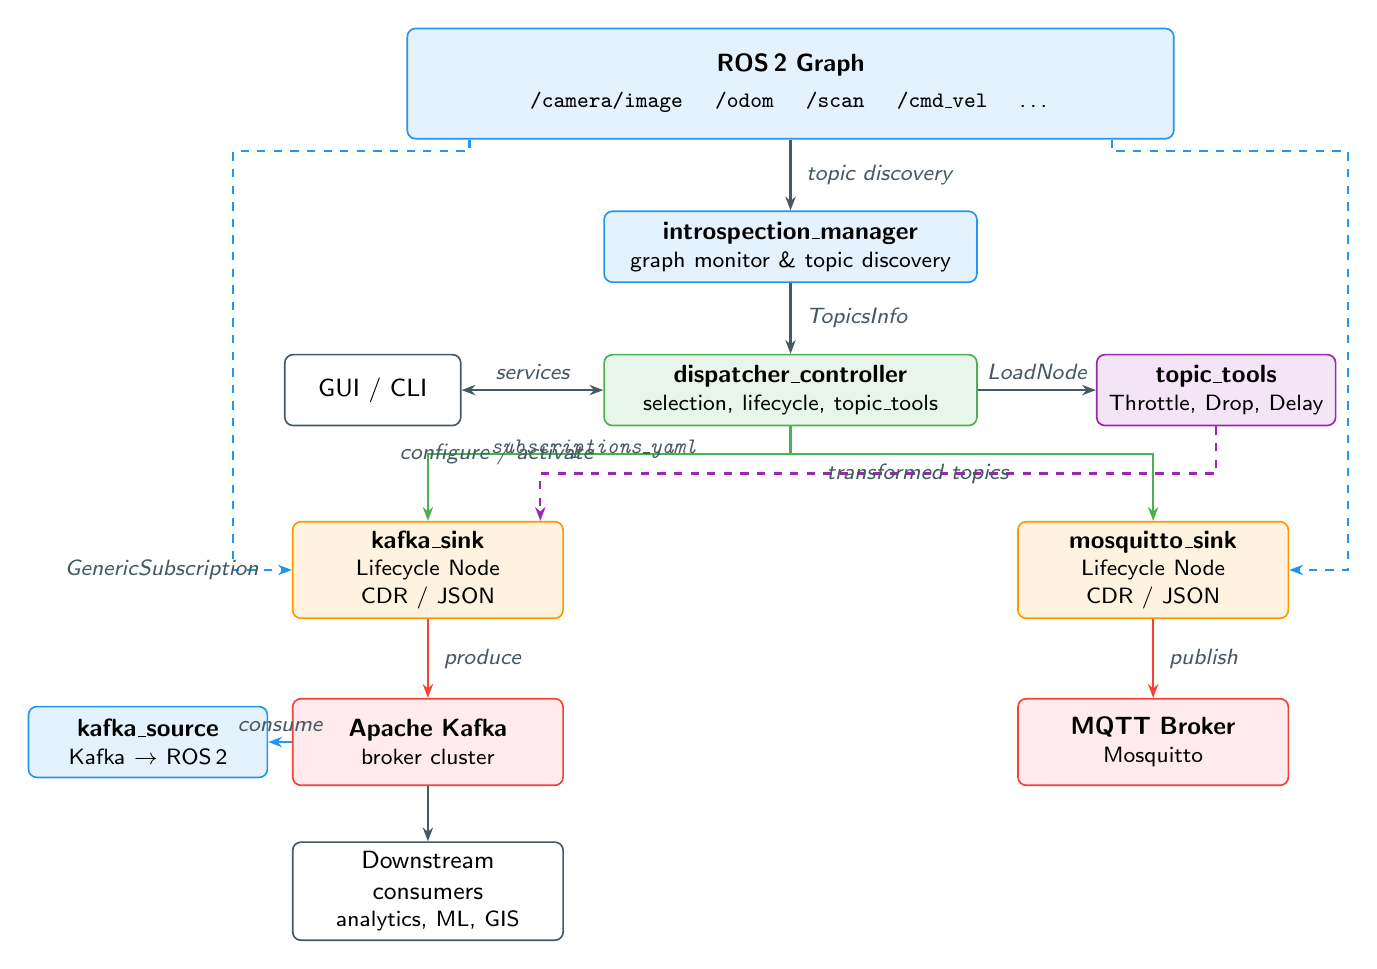
\begin{tikzpicture}[
    node distance=0.9cm and 1.2cm,
    >={Stealth[length=5pt]},
    every node/.style={font=\sffamily\small},
    box/.style={
        draw, rounded corners=3pt, minimum height=0.9cm,
        text width=#1, align=center, line width=0.6pt
    },
    box/.default=3.2cm,
    label node/.style={font=\sffamily\footnotesize\itshape, text=arrowgray},
]

% === ROS 2 Graph ===
\node[box=9.5cm, fill=ros2light, draw=ros2blue, minimum height=1.4cm] (graph)
    {\textbf{ROS\,2 Graph}\\[2pt]
     {\footnotesize\texttt{/camera/image} \quad \texttt{/odom} \quad \texttt{/scan} \quad \texttt{/cmd\_vel} \quad \ldots}};

% === Introspection Manager ===
\node[box=4.5cm, fill=ros2light, draw=ros2blue, below=0.9cm of graph] (intro)
    {\textbf{introspection\_manager}\\[-1pt]
     {\footnotesize graph monitor \& topic discovery}};

% === Dispatcher Controller ===
\node[box=4.5cm, fill=ctrllight, draw=ctrlgreen, below=0.9cm of intro] (ctrl)
    {\textbf{dispatcher\_controller}\\[-1pt]
     {\footnotesize selection, lifecycle, topic\_tools}};

% === GUI / CLI ===
\node[box=2.0cm, fill=white, draw=arrowgray, left=1.8cm of ctrl] (gui)
    {GUI / CLI};

% === Topic Tools ===
\node[box=2.8cm, fill=toollight, draw=toolpurple, right=1.5cm of ctrl] (tools)
    {\textbf{topic\_tools}\\[-1pt]
     {\footnotesize Throttle, Drop, Delay}};

% === Kafka Sink ===
\node[box=3.2cm, fill=sinklight, draw=sinkamber, below left=1.2cm and 0.5cm of ctrl] (ksink)
    {\textbf{kafka\_sink}\\[-1pt]
     {\footnotesize Lifecycle Node}\\[-1pt]
     {\footnotesize CDR / JSON}};

% === Mosquitto Sink ===
\node[box=3.2cm, fill=sinklight, draw=sinkamber, below right=1.2cm and 0.5cm of ctrl] (msink)
    {\textbf{mosquitto\_sink}\\[-1pt]
     {\footnotesize Lifecycle Node}\\[-1pt]
     {\footnotesize CDR / JSON}};

% === Kafka Broker ===
\node[box=3.2cm, fill=brokerlight, draw=brokerred, below=1.0cm of ksink, minimum height=1.1cm] (kafka)
    {\textbf{Apache Kafka}\\[-1pt]
     {\footnotesize broker cluster}};

% === MQTT Broker ===
\node[box=3.2cm, fill=brokerlight, draw=brokerred, below=1.0cm of msink, minimum height=1.1cm] (mqtt)
    {\textbf{MQTT Broker}\\[-1pt]
     {\footnotesize Mosquitto}};

% === Kafka Source (reverse path) ===
\node[box=2.8cm, fill=ros2light, draw=ros2blue, left=0.3cm of kafka] (ksource)
    {\textbf{kafka\_source}\\[-1pt]
     {\footnotesize Kafka $\to$ ROS\,2}};

% === Downstream ===
\node[box=3.2cm, fill=white, draw=arrowgray, below=0.7cm of kafka] (downstream)
    {Downstream consumers\\[-1pt]
     {\footnotesize analytics, ML, GIS}};

% ===== ARROWS =====

% Graph -> Introspection
\draw[->, thick, color=arrowgray]
    (graph.south) -- (intro.north)
    node[midway, right=2pt, label node] {topic discovery};

% Introspection -> Controller
\draw[->, thick, color=arrowgray]
    (intro.south) -- (ctrl.north)
    node[midway, right=2pt, label node] {TopicsInfo};

% GUI <-> Controller
\draw[<->, thick, color=arrowgray]
    (gui.east) -- (ctrl.west)
    node[midway, above, label node] {services};

% Controller -> Topic Tools
\draw[->, thick, color=arrowgray]
    (ctrl.east) -- (tools.west)
    node[midway, above, label node] {LoadNode};

% Controller -> Kafka Sink
\draw[->, thick, color=ctrlgreen]
    (ctrl.south) -- ++(0,-0.35) -| (ksink.north)
    node[pos=0.25, left=2pt, label node] {configure / activate};

% Controller -> Mosquitto Sink
\draw[->, thick, color=ctrlgreen]
    (ctrl.south) -- ++(0,-0.35) -| (msink.north)
    node[pos=0.25, right=2pt, label node] {};

% Graph -> Sinks (subscriptions - dashed)
\draw[->, thick, dashed, color=ros2blue]
    (graph.south west) ++(0.8,0) -- ++(0,-0.15) -- ++(-3.0,0) |- (ksink.west)
    node[pos=0.85, left=2pt, label node] {GenericSubscription};

\draw[->, thick, dashed, color=ros2blue]
    (graph.south east) ++(-0.8,0) -- ++(0,-0.15) -- ++(3.0,0) |- (msink.east)
    node[pos=0.85, right=2pt, label node] {};

% Kafka Sink -> Kafka
\draw[->, thick, color=brokerred]
    (ksink.south) -- (kafka.north)
    node[midway, right=2pt, label node] {produce};

% Mosquitto Sink -> MQTT
\draw[->, thick, color=brokerred]
    (msink.south) -- (mqtt.north)
    node[midway, right=2pt, label node] {publish};

% Kafka -> Kafka Source (reverse)
\draw[->, thick, color=ros2blue]
    (kafka.west) -- (ksource.east)
    node[midway, above, label node] {consume};

% Kafka -> Downstream
\draw[->, thick, color=arrowgray]
    (kafka.south) -- (downstream.north);

% Topic tools -> sinks (dashed, transformed topics)
\draw[->, thick, dashed, color=toolpurple]
    (tools.south) -- ++(0,-0.6) -| ($(ksink.north east)+(-0.3,0)$)
    node[pos=0.3, right=2pt, label node] {transformed topics};

% === YAML label on controller->sink arrows ===
\node[label node, below=0.05cm of ctrl, xshift=-2.5cm] {\texttt{subscriptions\_yaml}};

\end{tikzpicture}
\end{document}
